%% Common template of the research article using elsarticle-ru class.
%% The elsarticle-ru class is russian translation of the original elsarticle class provided by Elseiver (see http://www.elsevier.com/author-schemas/latex-instructions).
%% 
%% Author: Dmitriy O. Afanasyev
%% Email: dmafanasyev@gmail.com
%% Web: http://dmafanasyev.ru
%% Version: 1.0, Feb 04, 2015
%% 
%% ---------------------------------------------
%% 
%% It may be distributed under the conditions of the LaTeX Project Public
%% License, either version 1.2 of this license or (at your option) any
%% later version.  The latest version of this license is in
%%    http://www.latex-project.org/lppl.txt
%% and version 1.2 or later is part of all distributions of LaTeX
%% version 1999/12/01 or later.
%%

\documentclass[3p,11pt,authoryear]{elsarticle-ru}
\usepackage[T2A]{fontenc}
\usepackage[utf8]{inputenc}
\usepackage[russian]{babel}
\usepackage{epstopdf,cmap,amssymb,amsfonts,amsmath,mathtext,enumerate,float,natbib,indentfirst,hyperref,graphicx,multirow,setspace}
% pscyr used for good quality russian font rendering. See http://blog.harrix.org/?p=444 for the full installing instruction of pscyr. 
\usepackage{pscyr}

\graphicspath{{figures/ru/}}

\journal{Название журнала}

\begin{document}

\begin{frontmatter}

%% title, authors, affilations
%% title
\title{The algorithm of automatic gain quadrature signal module's working\tnoteref{titlenote}}
\tnotetext[titlenote]{This article is a start for development IP- module of automatic gain quadrature signal, namely, the device, resulting in an average level is an arbitrary signal to the desired at a predetermined time interval. The device is intended for using in Vivado package and is focused on the implementation on the basis of FPGA logic programming company Xilinx family - 7.}

%% authors & affiliations
\author[addr1]{Rodina Lera\corref{corrauthor}}
\cortext[corrauthor]{Master student, group 13541/4.}
\ead{email\_valeriarodina@ya.ru}
\ead[url]{http://github.com/valeryrodina/InfoSec}

%%\author[addr1,addr2]{Name of Author 2}
%%\ead{email\_author2@domen.ru}

\address[addr1]{Peter the Great St.Petersburg Polytechnic University}
\address[addr2]{Institute of Computer Science and Technology}


%% abstract
\begin{abstract}
Здесь дается краткая аннотация, характеризующая главную проблематику исследования, а также наиболее значимые полученные результаты.
\end{abstract}

%% keywords
\begin{keyword}
ключевое слово 1 \sep ключевое слово 2 \sep ключевое слово 3
\end{keyword}

\end{frontmatter}

%% main text
\section{Введение}
\label{sec:Intro}

Здесь необходимо обосновать актуальность темы работы, обозначить основную проблематику, а также дать краткий обзор предшествующих работ по данной тематике и результатов, полученных в них. Пример ссылок в гарвардском стиле выглядит так: \citet{bib:AuthorYear}.

Общепринятым завершением данного раздела служит следующий текст:

Дальнейший часть статьи организована следующим образом. В разделе~\ref{sec:Method} мы рассмотрим методологию исследования. В разделе~\ref{sec:Data} будет дана краткая характеристика используемых данных. Раздел~\ref{sec:Results} будет посвящен анализу результатов. Завершит работу раздел~\ref{sec:Conclusion}, в котором буду сделаны основные выводы.

\section{Методология}
\label{sec:Method}

В этом разделе описывается методология исследования.

\subsection{Название параграфа}
\label{sec:}

Пример простой формулы:

\begin{equation}\label{eq:eq_descr_1}
f(x) = ax+b
\end{equation}

\subsection{Название параграфа}
\label{sec:}

Пример более сложной формулы:
\begin{eqnarray}\label{eq:eq_descr_2}
f_{GND}(0, \sigma, k) = \frac{\phi(y)}{\sigma - k P_t},\\
y = \left\{
\begin{array}{ll}
 -\frac{1}{k} \log \left[  1 - \frac{k P_t}{\sigma} \right], & k \neq 0 \\
  \frac{P_t}{\sigma}, & k = 0
\end{array}
\right.\nonumber,
\end{eqnarray}

\section{Данные}
\label{sec:Data}

В этом разделе приводится описание использованных в работе данных, обосновывается их выбор, а также указываются источники их получения. Общераспространенной практикой является анализ описательной статистики, позволяющей сделать какие-то предположения еще до получения результатов исследования.

\section{Results}
\label{sec:Results}

This section presents the main results obtained in this research, as well as their detailed analysis is performed.

\subsection{Subsection name}
\label{sec:}

\begin{table*}[!h]
\caption{An example of a simple table containing descriptive statistics.}
\label{tab:tab_descr_1}
\setlength{\arrayrulewidth}{1.05 pt}
\renewcommand{\arraystretch}{1.1}
\begin{tabular*}{1.0\textwidth}{@{\extracolsep{\fill}}lrr}
\hline
Parameter & Column Name & Column Name \\
\hline
Mean, $\mu$ & 0.79 & 0.98 \\
\hline
\end{tabular*}
\begin{spacing}{0.5}
{\scriptsize Note: There are explanations to the table.}
\end{spacing}
\end{table*}

\subsection{Subsection name}
\label{sec:}

\begin{table*}[!h]
\caption{An example of more complicated table containing estimates of the model parameters.}
\label{tab:}
\setlength{\arrayrulewidth}{1.05 pt}
\renewcommand{\arraystretch}{1.1}
\begin{tabular*}{1.0\textwidth}{@{\extracolsep{\fill}}lrrr}
\hline
Parameter & \textit{Column Name} & \textit{Column Name} & \textit{Column Name} \\
\hline

\multicolumn{4}{l}{\textit{Group Name}} \\
$\mu$ & 0.30\textsuperscript{***} {\footnotesize (0.01)} & 0.30\textsuperscript{***} {\footnotesize (0.01)} & 0.30\textsuperscript{***} {\footnotesize (0.01)} \\
$\phi$ & 0.30\textsuperscript{***} {\footnotesize (0.01)} & 0.30\textsuperscript{***} {\footnotesize (0.01)} & 0.30\textsuperscript{***} {\footnotesize (0.01)} \\

\multicolumn{4}{l}{\textit{Group Name}} \\
$\mu$ & 0.40\textsuperscript{*} {\footnotesize (0.17)} & 0.40\textsuperscript{*} {\footnotesize (0.17)} & 0.40\textsuperscript{*} {\footnotesize (0.17)} \\
$\phi$ & 0.40\textsuperscript{*} {\footnotesize (0.17)} & 0.40\textsuperscript{*} {\footnotesize (0.17)} & 0.40\textsuperscript{*} {\footnotesize (0.17)} \\

\hline
\end{tabular*}
\begin{spacing}{0.5}
{\scriptsize Note: Standard errors of coefficients are given in parentheses. The levels of significance notation: *** -- 1\%, ** -- 5\%, * -- 10\%.}
\end{spacing}
\end{table*}

\subsection{Subsection name}
\label{sec:}

%%\begin{figure*}[!h]
%%\centering
%%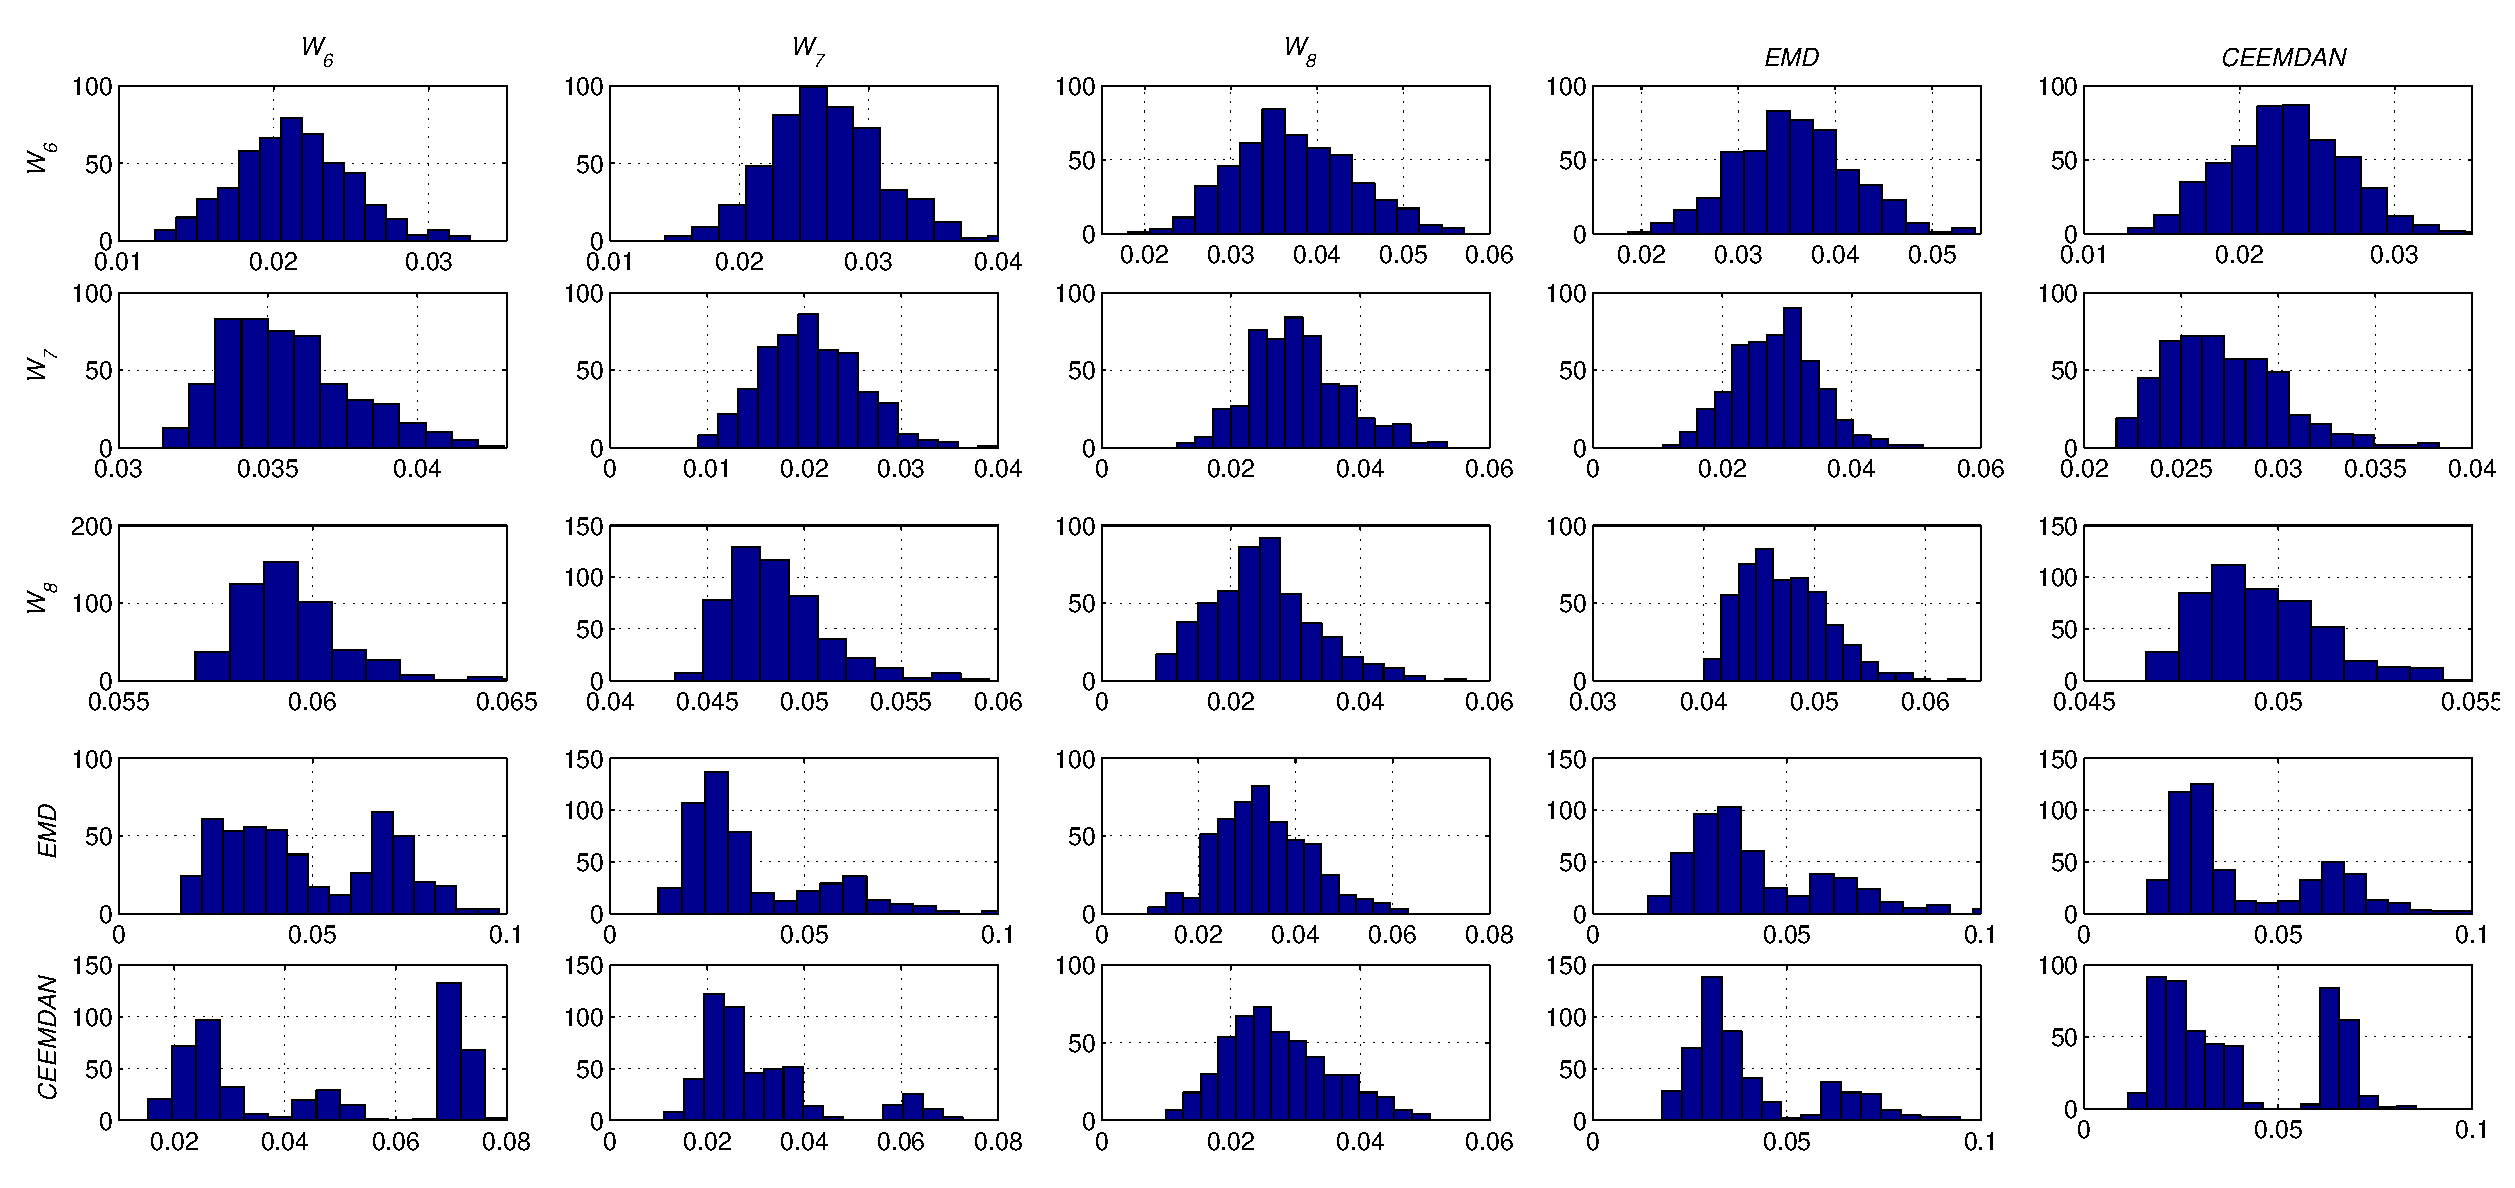
\includegraphics[width=1.0\textwidth,keepaspectratio]{Figure}
%%\caption{Figure Title.}
%%\label{fig:}
%%\end{figure*}

\section{Заключение}
\label{sec:Conclusion}

В данном разделе обобщаются полученные результаты и делаются основные выводы исследования.

\section{Acknowledgements}
\label{sec:Acknowledgement}

Section gives acknowledgments to people or organizations that have provided substantial assistance to the article.

As a base, you can use the following template:

The authors are grateful to \{name\} for his fruitful comments on the text of the
paper. Responsibility for all errors and inaccuracies made by the authors rests solely on the part of
the authors.

\appendix
\section{Appendix Name}
\label{sec:Appendix_}

Here is content of the work appendix. In the general case there are more than one appendixes.

%% bibliography
\phantomsection
\addcontentsline{toc}{section}{Список литературы}
\section*{Список литературы}
\bibliographystyle{elsarticle-harv-ru}
\bibliography{biblio}
\end{document}